\documentclass[%
12pt, %
final, % 
oneside, % 
onecolumn, %  
centertags]{article} % относится к классу article и размер шрифта 12 пунктовб, {article: статья, report: отчеты и диссертации, book: книга, letter: письмо}

% \usepackage{fontspec}
 
% \setmainfont{Times New Roman}

% \documentclass[a4paper, 12pt]{report}

\topmargin= -30pt % насколько сверху будет страница
\textheight= 650pt


\usepackage[utf8]{inputenc} % задает кодировку, utf-8 кодировка, включающая в себя знаки почти всех языков мира
\usepackage[english]{babel} % подключает необходимые языки, основным языком является английский

\selectlanguage{english} % настройки будут на английском, но писать будет на русском

\usepackage{euscript}
\usepackage{supertabular}

\renewcommand{\baselinestretch}{1.0} 

\usepackage[colorlinks=true,linkcolor=blue,unicode=true,urlcolor = blue]{hyperref} %hypered
\usepackage[pdftex]{graphicx} % для графики

\usepackage{amsthm, amssymb, amsmath, amsfonts} % математический пакет, математические шрифты
\usepackage{textcomp}
\usepackage[noend]{algorithmic}
\usepackage[ruled]{algorithm}
\usepackage{lipsum}
\usepackage{indentfirst}
\usepackage{babel}
\usepackage{pgfplots}
\usepackage{setspace}
\usepackage{xcolor}
\usepackage{hyperref}
\usepackage{subfigure}

\setcounter{secnumdepth}{5}
\setcounter{tocdepth}{5}
\newcommand\simpleparagraph[1]{%
  \stepcounter{paragraph}\paragraph*{\theparagraph\quad{}#1}}
\usepackage{listings}
% \usepackage{xcolor}
%\usepackage{minted}

\lstset { %
     language=C++,
     backgroundcolor=\color{black!5}, % set backgroundcolor
     basicstyle=\footnotesize,% basic font setting
}


\linespread{1.0} 
\setlength{\parindent}{2.4em}
\setlength{\parskip}{0.1em}

\pgfplotsset{compat=1.9}
\pgfplotsset{model/.style = {blue, samples = 100}} 
\pgfplotsset{experiment/.style = {red}}

\theoremstyle{plain}
\binoppenalty=10000

\newtheorem{theorem}{Theorem}[section] % theorem

\theoremstyle{definition}
% \newtheorem{definition}{Определение}[subsection]
\newtheorem{definition}{Definition}[subsection]

\theoremstyle{remark}
% \newtheorem{remark}{Замечание}[section]

% \newtheorem{corollary}{Следствие}

% \newtheorem{proposition}{Proposition}

% \newtheorem{example}{Пример}

% \newtheorem{lemma}{Лемма}[section]

\renewcommand*{\proofname}{Proof}

\graphicspath{ {./images/} }


% \usepackage{amsmath,amsfonts,amssymb, setspace}  % Разнообразные математические команды и значки
% \usepackage{indentfirst}     % Отступ в первом абзаце

% \pagestyle{empty}
\usepackage[left=2.5cm, right=1.5cm, top=2.5cm, bottom=2.5cm]{geometry}
\usepackage[medium]{titlesec}
\usepackage{graphicx}
% \graphicspath{ {./images/} }

\begin{document}

	\begin{titlepage} 
		\begin{center}
		\textbf{}\\[2.0cm]
		\LARGE FEDERAL STATE AUTONOMOUS EDUCATIONAL INSTITUTION OF HIGHER EDUCATION \\[0.5cm]
		\Large ITMO UNIVERSITY \\[3cm]
		\LARGE Report\\
		\Large MPI. Assignments $10-11$ \\
		\Large Parallel algorithms for the analysis and synthesis of data \\[4cm]


		\begin{flushright}
		Performed by\\
		Aleksandr Shirokov\\
		J4133c\\
		Accepted by\\
		Petr Andriushchenko

		Deadline: 21.12.21
		\end{flushright}

		\vfill 

		{\Large {St. Petersburg}} \par
		{\Large {2021}}
		\end{center} 
	\end{titlepage}

\tableofcontents
\newpage


\section{Assignments}

\subsection{Assignment 9. MPI. MPI\_Reduce.}

\subsubsection{Formulation of the problem}

\begin{enumerate}
	\item Write an MPI program in which the global vector addition operation is modeled by a 
doubling (cascade) scheme using point-to-point data transfers.
	\item Compare the execution time of such a simulation using the \textsc{MPI\_Reduce} procedure on as many processes as possible. Each process stores an array of $1,000,000$ elements equal to $1$.
\end{enumerate}

\begin{center}
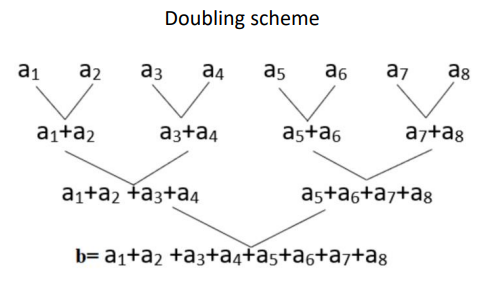
\includegraphics[scale=0.75]{9.double.png}
\end{center}

\textbf{MPI\_Reduce}

The \textsc{MPI\_Reduce} function concatenates the input buffer entries of each process in a group 
using the \textbf{op} operation and returns the concatenated value to the root process's output 
buffer.


int \textbf{MPI\_Reduce} (
\begin{itemize}
	\item IN void *\textbf{sendbuf} - address of the beginning of the input buffer;
	\item OUT void *\textbf{recvbuf} - address of the beginning of the result buffer (used only in the receiving 
process root);
	\item IN int \textbf{count} - the number of elements in the input buffer;
	\item IN MPI\_Datatype \textbf{sendtype} - the type of elements in the input buffer;
	\item IN MPI\_Op \textbf{op} - the operation by which the reduction is performed;
	\item IN int \textbf{root} - number of the receiving process of the operation result;
	\item IN MPI\_Comm \textbf{comm} - communicator
\end{itemize}
)

\subsubsection{Example of launch parameters and output. Detailed description of solution}

Code for \textbf{assignment 9} is \href{https:\//github.com/aptmess/parallel_algorithms/blob/master/HT/hw_mpi/Assignment9.c}{here}.

Compilation example: \textsc{mpic++ -o ./cpf/9.o Assignment9.c}

Launch example, there are two options: 
\begin{enumerate}
	\item \textsc{mpirun --oversubscribe -np 16 ./cpf/9.o 100000000 double}
	\item \textsc{mpirun --oversubscribe -np 16 ./cpf/9.o 100000000 reduce}
\end{enumerate}

\begin{center}
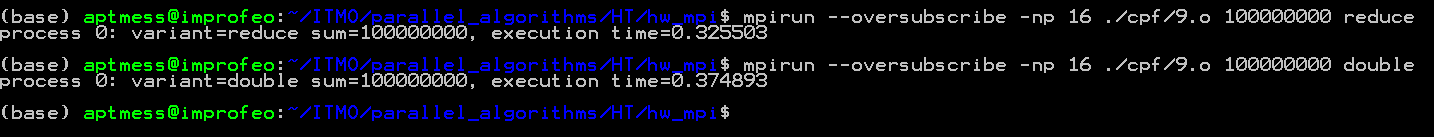
\includegraphics[scale=0.48]{9.png}

Results
\end{center}

Let's move to the the code and explain how it works.

\begin{figure}[h!]
\centering
\subfigure{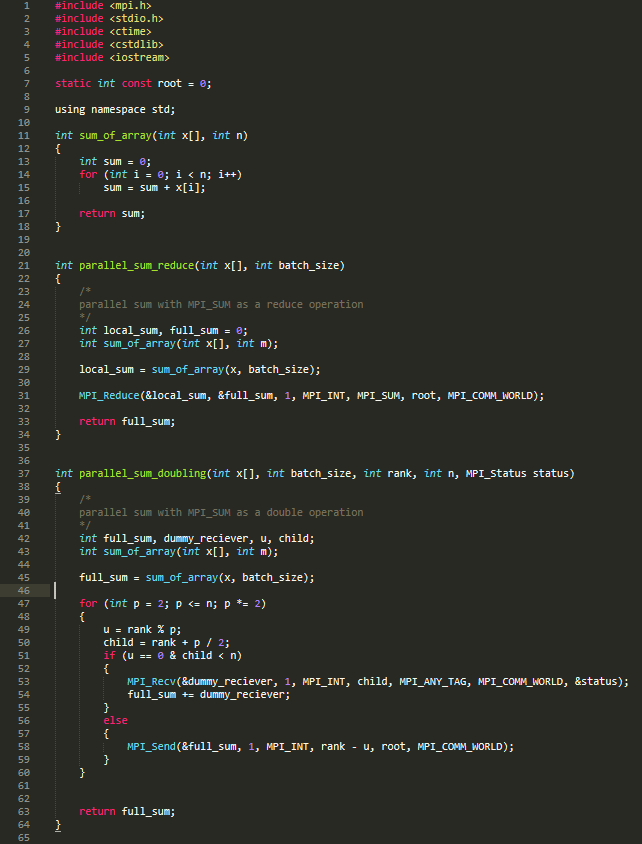
\includegraphics[width=0.47\textwidth]{9.1.code.png}} 
\subfigure{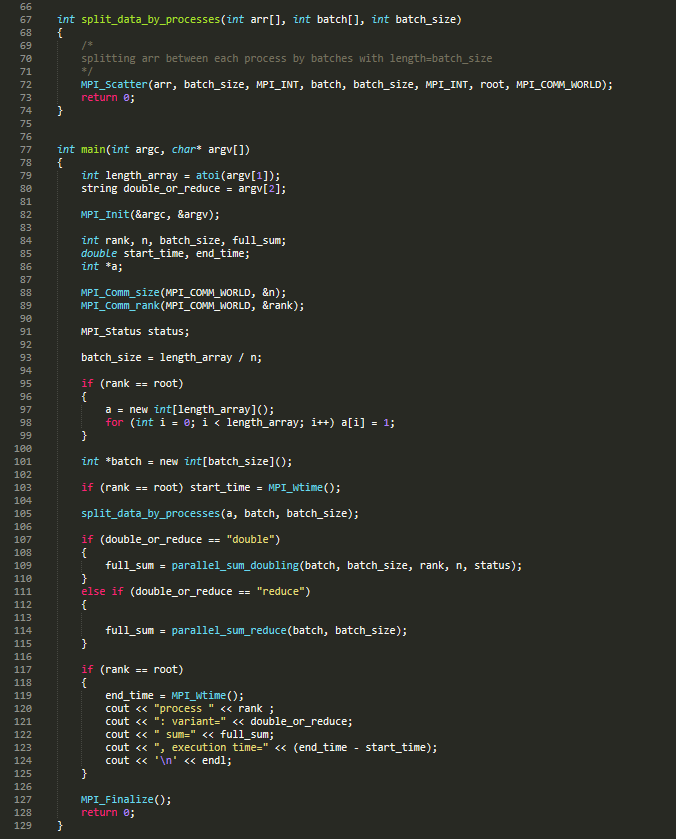
\includegraphics[width=0.5\textwidth]{9.2.code.png}} 

Assignment9 code
\end{figure}

In this code there are two functions base functions - \textsc{parallel\_sum\_reduce} and \textsc{parallel\_sum\_doubling}. In first function we are for each process and for their part of input array compute sum and send the result to toor process using syntax of \textsc{MPI\_Reduce}, in \textsc{parallel\_sum\_doubling} function we are splitting our workers as a tree (amount of processes should be a degree of $2$ because of implemenation condition). After that if there are a way to split worker to more workers less than amount of processes we are splitting and waiting for result of each child process, else we are sending sum - the structure as on picture in the previous subsection. In main functions we initialise array of ones, with function \textsc{MPI\_Scatter} send for each process their own part of array and depending on input parameter counting the sum. After some expereiements I mentioned that reduce operation worke quicklier than doubling (as we can see in picture \textsc{Results}).



\subsection{Appendix}

The link to the sourse code which is placed on my \href{https://github.com/aptmess/parallel_algorithms}{github}.


\end{document}